\section{Circuits}
\begin{figure}
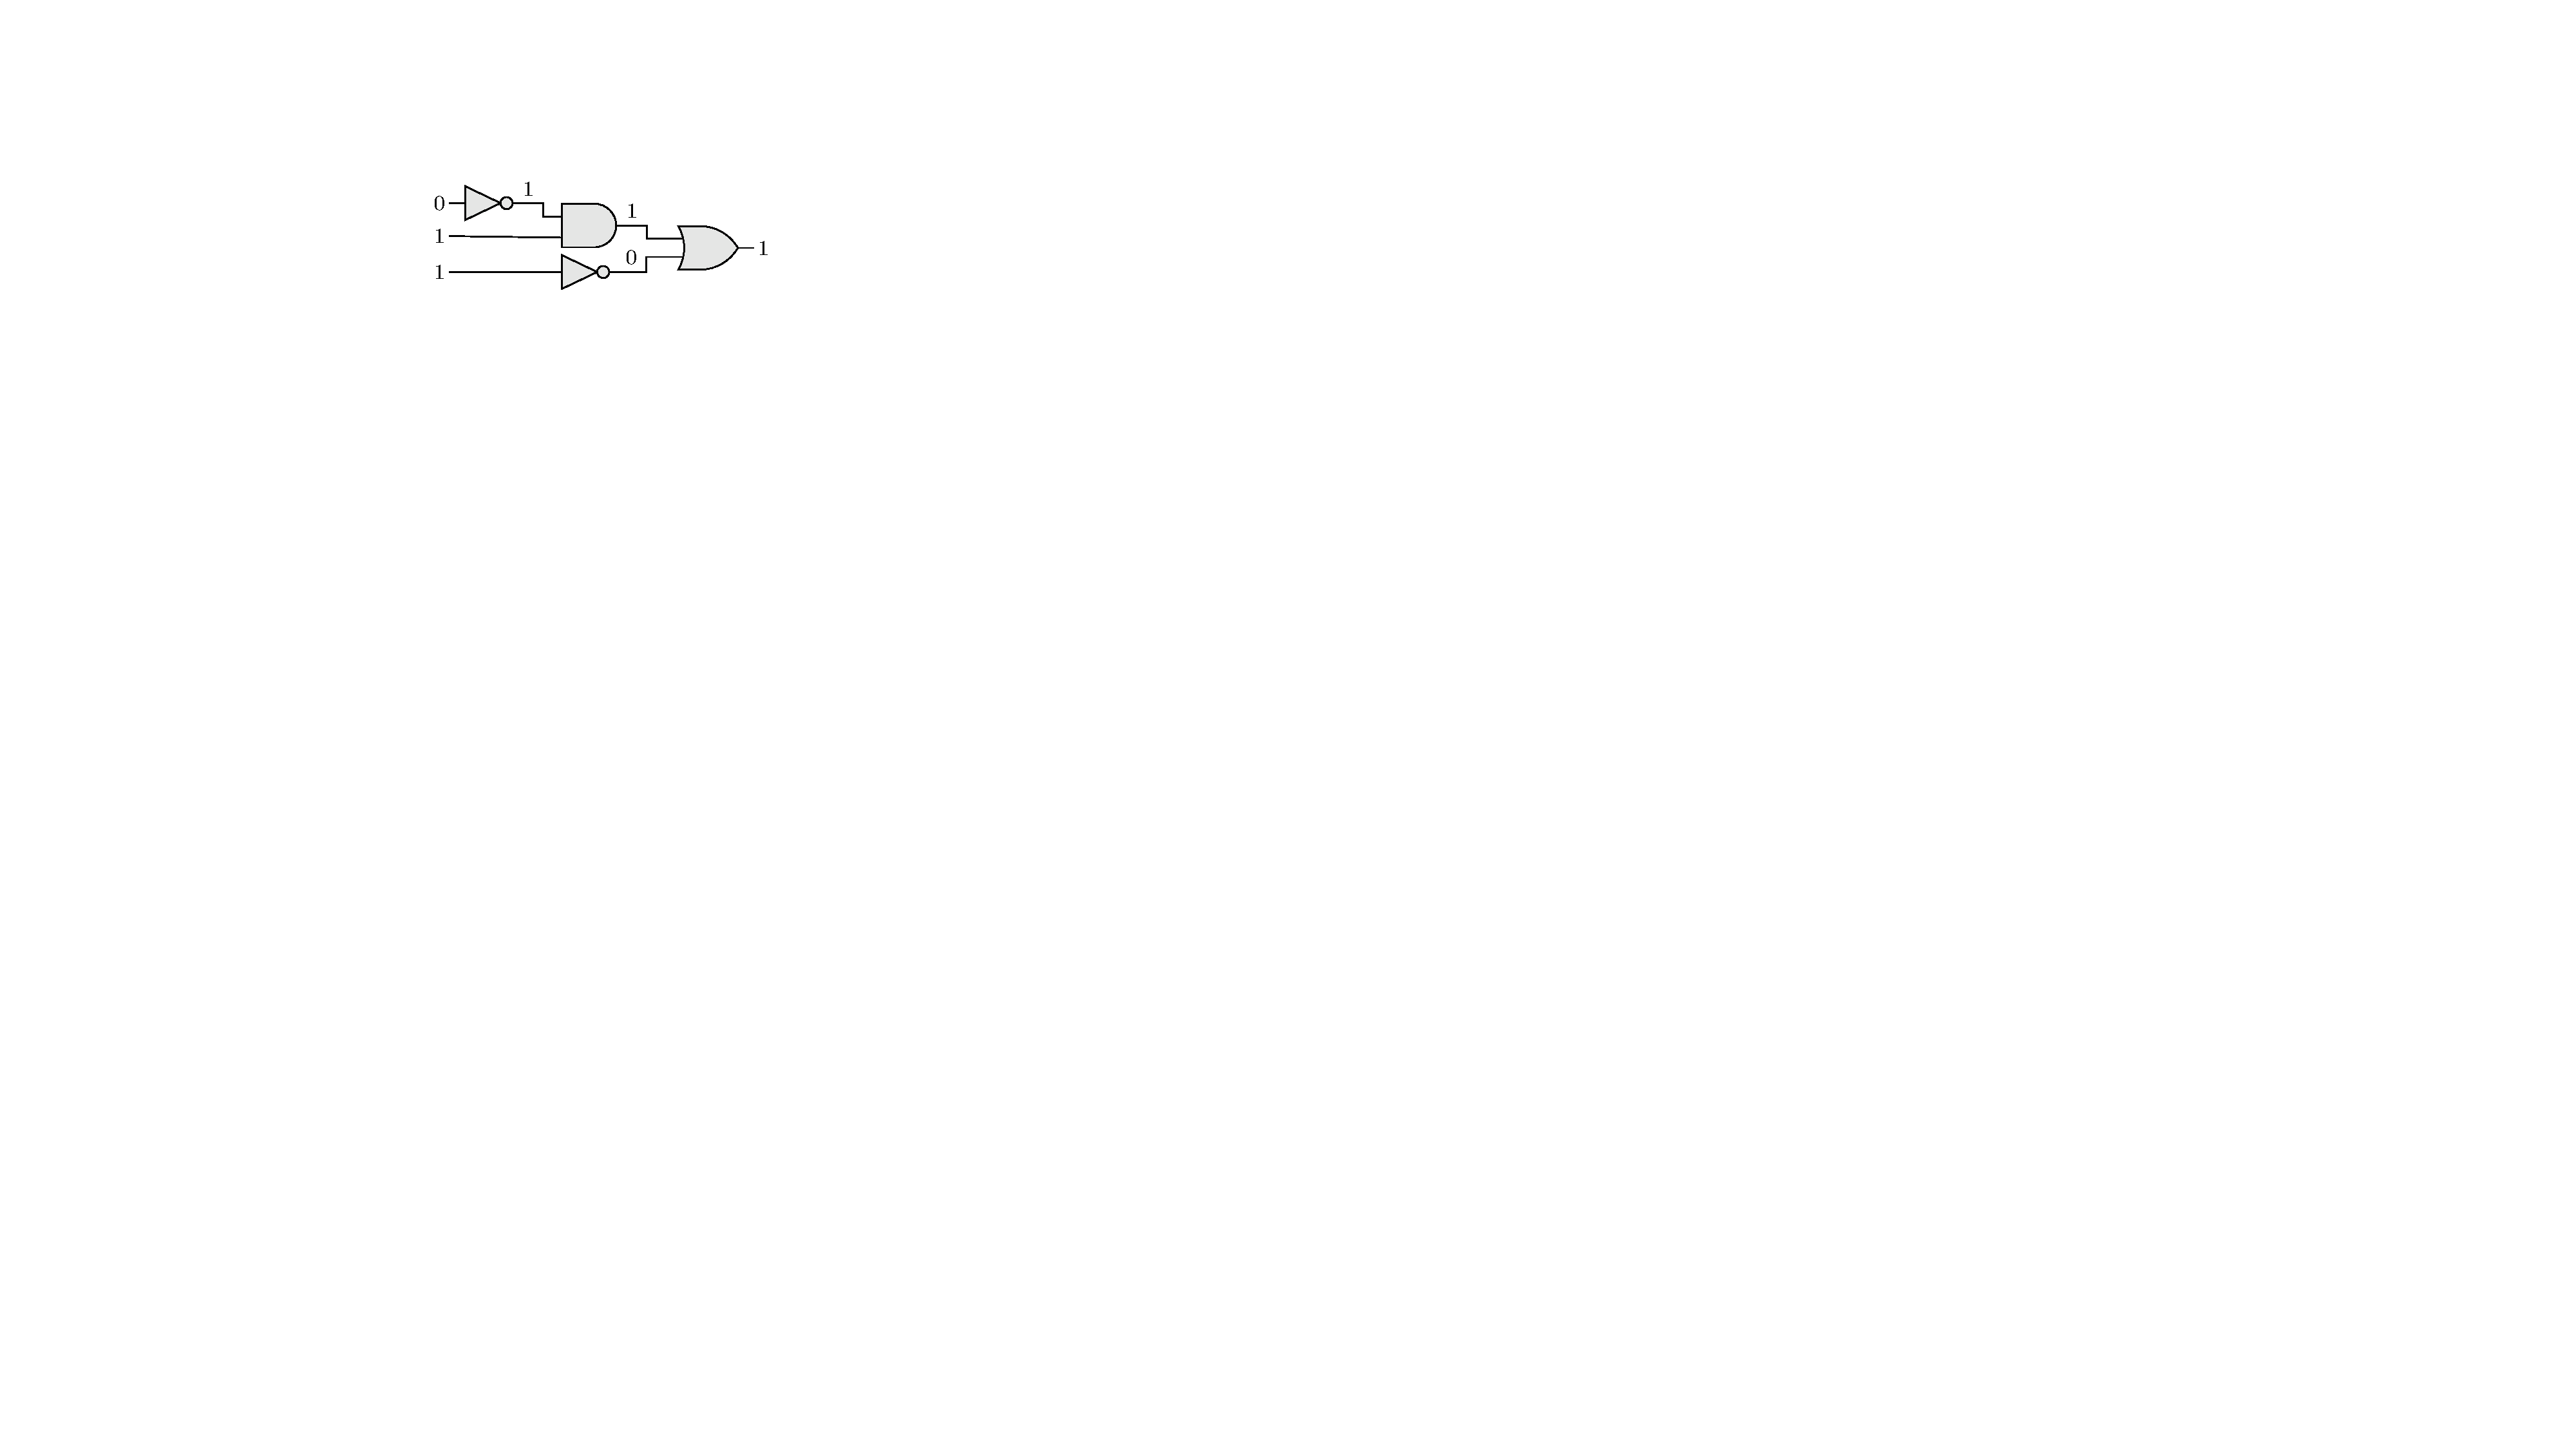
\includegraphics[]{Figures/HWCircuits/DigitalCircuit}
\end{figure}
I convention a circuits, we store information as sets of {\it bits} with values $0$ and $1$.
%
The basic data transformer is a Boolean {\it gate}.
%
We can see a gate as a Boolean function taking a sequence of Binary bits as input, and producing an output bit as output.
%
A combinatorial circuit consists of set of gates and can also been as Boolean function.
%
The circuits takes a sequence of bits as input and a produces a sequence of bits as output.
%
Typically, we also have a set of internal bits that represent the connection between gate
%
In \cref{a}, the circuit has three input bits,  one output bit, and three internal bits.

Often, we consider the {\it state} of a sequence of bits by giving the sequence of their values.
%
For instance, the input state in \cref{a} is $011$ since the three input bits have values $0$, $1$, and $1$ in that order.
%
We observe that the set of the input states in this case is of size $8$: in general, $n$ bits may have $2^n$ possible states.
